\documentclass[11pt,tikz]{standalone}
\usepackage{eulervm}
\usepackage{libertine}
%\usepackage{amsmath}

% ------- %
% Colours %
% ------- %

% Playroom colour scheme
% http://www.colourlovers.com/palette/1047246/Playroom
\definecolor{PeelingPaper}{RGB}{5,135,137}
\definecolor{WoodenPlatforms}{RGB}{80,61,46}
\definecolor{Puzzle24000}{RGB}{213,75,26}
\definecolor{Escape}{RGB}{227,167,47}

%% u.make.me.happy colour scheme
%% http://www.colourlovers.com/palette/360922/u.make.me.happy
%\definecolor{Amelllatoo}{HTML}{5CACC4}
%\definecolor{Lmao}{HTML}{8CD19D}
%\definecolor{UFunny}{HTML}{CEE879}
%\definecolor{FairyStream}{HTML}{FCB653}
%\definecolor{Hexy}{HTML}{FF5254}

%% Mongo for Mormons colour scheme
%% http://www.colourlovers.com/palette/324775/Mangos_for_Mormons
%\definecolor{Murky}{HTML}{595643}
%\definecolor{Everything}{HTML}{4E6B66}
%\definecolor{Melon}{HTML}{ED834E}
%\definecolor{TheHolyGrail}{HTML}{EBCC6E}

%% Chick Mellow colour scheme
%% http://www.colourlovers.com/palette/254301/[Chic]_-_Mellow
%\definecolor{Gemma}{HTML}{11644D}
%\definecolor{MellowMeadow}{HTML}{A0B046}
%\definecolor{TheKingsCrown}{HTML}{F2C94E}
%\definecolor{MellowMe}{HTML}{F78145}
%\definecolor{AlmostZeroZero}{HTML}{F24E4E}

% Other colours I use
\definecolor{Tropiteal}{RGB}{0,168,198}
\definecolor{TealDrop}{RGB}{64,192,203}
\definecolor{WhiteTrash}{RGB}{249,242,231}
\definecolor{AtomicBikini}{RGB}{174,226,57}
\definecolor{FeebleWeek}{RGB}{143,190,0}
\definecolor{ICantExpress}{RGB}{28,20,13}
\definecolor{Marty}{RGB}{250,42,0}
\definecolor{WeddedPassion}{RGB}{164,7,120}


\colorlet{ColourBase}{PeelingPaper}
\colorlet{ColourHl1}{Puzzle24000}
\colorlet{ColourHl2}{FeebleWeek}
\colorlet{ColourHl3}{Escape}
\colorlet{ColourDark}{WoodenPlatforms}

\newcommand{\ColBaseText}{blue}
\newcommand{\ColHlIText}{red}



\usetikzlibrary{decorations.text}
\usetikzlibrary{arrows.meta}


\begin{document}
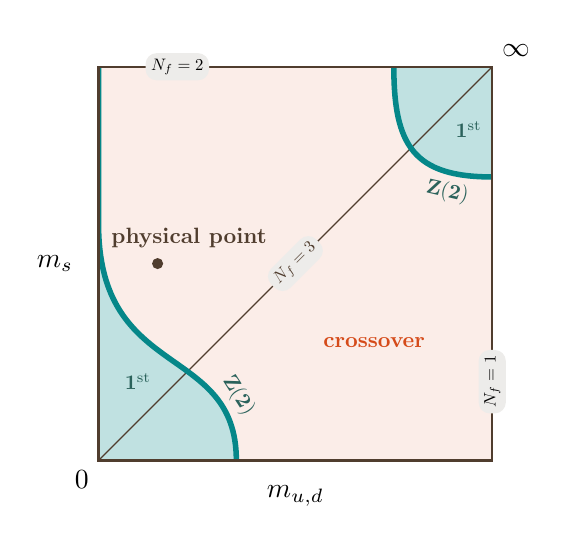
\begin{tikzpicture}

  \fill[ColourHl1!10] (0,0) rectangle (5cm,5cm);

  \begin{scope}
    \clip (0,0) rectangle (5cm,5cm);
    \fill[ColourBase!25] (0,5cm) -- (0,3cm) .. controls +(0,-2cm) and +(0,1.5cm) .. (1.75cm,0) -- (0,0) -- cycle;
    \fill[ColourBase!25]  (3.75cm,5cm) .. controls +(0,-1cm) and +(-1cm,0) .. (5cm,3.6cm) -- (5cm,5cm) -- cycle;

    \draw[ColourDark] (0,0) -- (5cm,5cm)
      node [midway,sloped,scale=0.6,fill=ColourDark!10,rounded corners] {$N_f = 3$};

    \draw[ColourBase,line width=2pt]  (0,5cm) -- (0,3cm) .. controls +(0,-2cm) and +(0,1.5cm) .. (1.75cm,0)
      node [sloped,pos=.8,above,scale=0.75,ColourBase!50!ColourDark] {$\mathbf{Z(2)}$};
    \draw[ColourBase,line width=2pt]  (3.75cm,5cm) .. controls +(0,-1cm) and +(-1cm,0) .. (5cm,3.6cm)
      node [sloped,pos=.8,below,scale=0.75,ColourBase!50!ColourDark] {$\mathbf{Z(2)}$};
  \end{scope}

  \fill [ColourDark] (.75cm,2.5cm) circle (2pt)
    node [above=.1cm, scale=0.8,xshift=.5cm,font=\bfseries] {physical point};

  \draw[ColourDark,thick] (0,0) -- (5cm,0) -- (5cm,5cm) -- (0,5cm) -- cycle;

  \node[scale=0.6,fill=ColourDark!10,rounded corners] at (1cm,5cm) {$N_f = 2$};
  \node[scale=0.6,fill=ColourDark!10,rounded corners,rotate=90] at (5cm,1cm) {$N_f = 1$};

  \node[anchor=north,scale=1.0] at (2.5cm, -.2cm) {$m_{u,d}$};
  \node[anchor=east,scale=1.0] at (-.2cm, 2.5cm) {$m_s$};
  \node[white,anchor=west,scale=0.6] at (5.2cm, 2.5cm) {$m_s$};
  \node[white,anchor=south,scale=0.6] at (2.5cm, 5.2cm) {$m_{u,d}$};

  \node[scale=0.8,ColourHl1,font=\bfseries] at (3.5cm,1.5cm) {crossover};
  \node[scale=0.75,ColourBase!50!ColourDark] at (0.5cm, 1cm) {$\mathbf{1^{\mathrm{st}}}$};
  \node[scale=0.75,ColourBase!50!ColourDark] at (4.7cm, 4.2cm) {$\mathbf{1^{\mathrm{st}}}$};

  \node[scale=1.0,anchor=north east] at (0,0) {0};
  \node[scale=1.0,anchor=south west] at (5cm,5cm) {$\infty$};

\end{tikzpicture}
\end{document}


